\documentclass{extbook}[14pt]
\usepackage{multicol, enumerate, enumitem, hyperref, color, soul, setspace, parskip, fancyhdr, amssymb, amsthm, amsmath, latexsym, units, mathtools}
\everymath{\displaystyle}
\usepackage[headsep=0.5cm,headheight=0cm, left=1 in,right= 1 in,top= 1 in,bottom= 1 in]{geometry}
\usepackage{dashrule}  % Package to use the command below to create lines between items
\newcommand{\litem}[1]{\item #1

\rule{\textwidth}{0.4pt}}
\pagestyle{fancy}
\lhead{}
\chead{Answer Key for Progress Quiz 6 Version ALL}
\rhead{}
\lfoot{4563-7456}
\cfoot{}
\rfoot{Summer C 2021}
\begin{document}
\textbf{This key should allow you to understand why you choose the option you did (beyond just getting a question right or wrong). \href{https://xronos.clas.ufl.edu/mac1105spring2020/courseDescriptionAndMisc/Exams/LearningFromResults}{More instructions on how to use this key can be found here}.}

\textbf{If you have a suggestion to make the keys better, \href{https://forms.gle/CZkbZmPbC9XALEE88}{please fill out the short survey here}.}

\textit{Note: This key is auto-generated and may contain issues and/or errors. The keys are reviewed after each exam to ensure grading is done accurately. If there are issues (like duplicate options), they are noted in the offline gradebook. The keys are a work-in-progress to give students as many resources to improve as possible.}

\rule{\textwidth}{0.4pt}

\begin{enumerate}\litem{
Construct the lowest-degree polynomial given the zeros below. Then, choose the intervals that contain the coefficients of the polynomial in the form $x^3+bx^2+cx+d$.
\[ -3 - 2 i \text{ and } -3 \]The solution is \( x^{3} +9 x^{2} +31 x + 39 \), which is option C.\begin{enumerate}[label=\Alph*.]
\item \( b \in [-5, 3], c \in [5.4, 6.45], \text{ and } d \in [7.9, 9.4] \)

$x^{3} + x^{2} +6 x + 9$, which corresponds to multiplying out $(x + 3)(x + 3)$.
\item \( b \in [-5, 3], c \in [4.58, 5.53], \text{ and } d \in [1.9, 7.1] \)

$x^{3} + x^{2} +5 x + 6$, which corresponds to multiplying out $(x + 2)(x + 3)$.
\item \( b \in [2, 13], c \in [30.15, 31.6], \text{ and } d \in [38.1, 39.8] \)

* $x^{3} +9 x^{2} +31 x + 39$, which is the correct option.
\item \( b \in [-17, -6], c \in [30.15, 31.6], \text{ and } d \in [-42, -38.7] \)

$x^{3} -9 x^{2} +31 x -39$, which corresponds to multiplying out $(x-(-3 - 2 i))(x-(-3 + 2 i))(x -3)$.
\item \( \text{None of the above.} \)

This corresponds to making an unanticipated error or not understanding how to use nonreal complex numbers to create the lowest-degree polynomial. If you chose this and are not sure what you did wrong, please contact the coordinator for help.
\end{enumerate}

\textbf{General Comment:} Remember that the conjugate of $a+bi$ is $a-bi$. Since these zeros always come in pairs, we need to multiply out $(x-(-3 - 2 i))(x-(-3 + 2 i))(x-(-3))$.
}
\litem{
Which of the following equations \textit{could} be of the graph presented below?

\begin{center}
    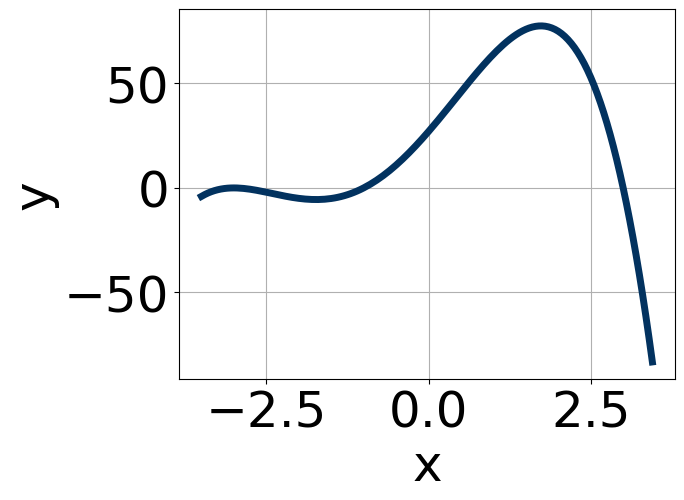
\includegraphics[width=0.5\textwidth]{../Figures/polyGraphToFunctionA.png}
\end{center}


The solution is \( -15(x + 3)^{10} (x - 3)^{7} (x + 1)^{11} \), which is option A.\begin{enumerate}[label=\Alph*.]
\item \( -15(x + 3)^{10} (x - 3)^{7} (x + 1)^{11} \)

* This is the correct option.
\item \( -9(x + 3)^{11} (x - 3)^{8} (x + 1)^{9} \)

The factor $-3$ should have an even power and the factor $3$ should have an odd power.
\item \( -7(x + 3)^{10} (x - 3)^{6} (x + 1)^{7} \)

The factor $(x - 3)$ should have an odd power.
\item \( 5(x + 3)^{10} (x - 3)^{5} (x + 1)^{4} \)

The factor $(x + 1)$ should have an odd power and the leading coefficient should be the opposite sign.
\item \( 7(x + 3)^{6} (x - 3)^{5} (x + 1)^{5} \)

This corresponds to the leading coefficient being the opposite value than it should be.
\end{enumerate}

\textbf{General Comment:} General Comments: Draw the x-axis to determine which zeros are touching (and so have even multiplicity) or cross (and have odd multiplicity).
}
\litem{
Which of the following equations \textit{could} be of the graph presented below?

\begin{center}
    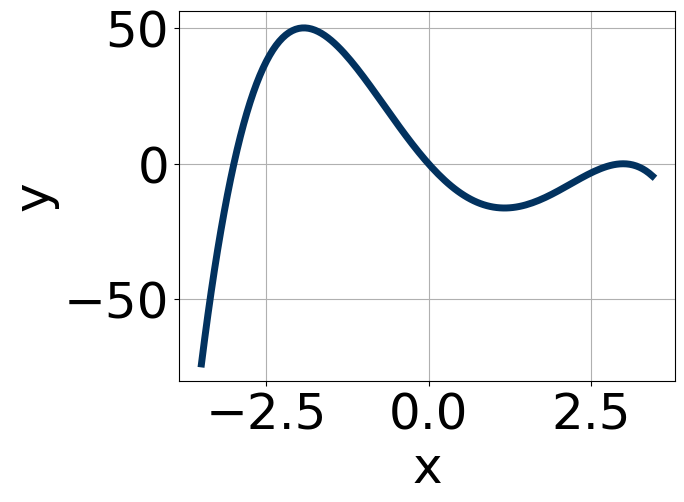
\includegraphics[width=0.5\textwidth]{../Figures/polyGraphToFunctionCopyA.png}
\end{center}


The solution is \( -7x^{7} (x - 3)^{8} (x + 3)^{5} \), which is option D.\begin{enumerate}[label=\Alph*.]
\item \( 10x^{7} (x - 3)^{4} (x + 3)^{10} \)

The factor $(x + 3)$ should have an odd power and the leading coefficient should be the opposite sign.
\item \( 15x^{11} (x - 3)^{6} (x + 3)^{5} \)

This corresponds to the leading coefficient being the opposite value than it should be.
\item \( -20x^{6} (x - 3)^{9} (x + 3)^{7} \)

The factor $3$ should have an even power and the factor $0$ should have an odd power.
\item \( -7x^{7} (x - 3)^{8} (x + 3)^{5} \)

* This is the correct option.
\item \( -18x^{4} (x - 3)^{4} (x + 3)^{5} \)

The factor $x$ should have an odd power.
\end{enumerate}

\textbf{General Comment:} General Comments: Draw the x-axis to determine which zeros are touching (and so have even multiplicity) or cross (and have odd multiplicity).
}
\litem{
Describe the zero behavior of the zero $x = 4$ of the polynomial below.
\[ f(x) = 2(x + 6)^{8}(x - 6)^{4}(x - 4)^{10}(x + 4)^{7} \]The solution is the graph below, which is option C.
    \begin{center}
        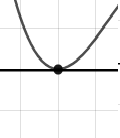
\includegraphics[width=0.3\textwidth]{../Figures/polyZeroBehaviorCopyCA.png}
    \end{center}\begin{enumerate}[label=\Alph*.]
\begin{multicols}{2}
\item 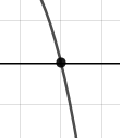
\includegraphics[width = 0.3\textwidth]{../Figures/polyZeroBehaviorCopyAA.png}
\item 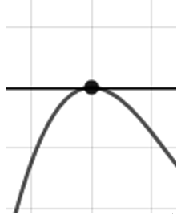
\includegraphics[width = 0.3\textwidth]{../Figures/polyZeroBehaviorCopyBA.png}
\item 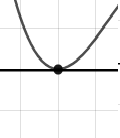
\includegraphics[width = 0.3\textwidth]{../Figures/polyZeroBehaviorCopyCA.png}
\item 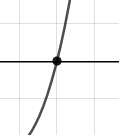
\includegraphics[width = 0.3\textwidth]{../Figures/polyZeroBehaviorCopyDA.png}
\end{multicols}\item None of the above.\end{enumerate}
\textbf{General Comment:} You will need to sketch the entire graph, then zoom in on the zero the question asks about.
}
\litem{
Construct the lowest-degree polynomial given the zeros below. Then, choose the intervals that contain the coefficients of the polynomial in the form $x^3+bx^2+cx+d$.
\[ 2 + 3 i \text{ and } 3 \]The solution is \( x^{3} -7 x^{2} +25 x -39 \), which is option D.\begin{enumerate}[label=\Alph*.]
\item \( b \in [4, 11], c \in [21.54, 25.63], \text{ and } d \in [33, 43] \)

$x^{3} +7 x^{2} +25 x + 39$, which corresponds to multiplying out $(x-(2 + 3 i))(x-(2 - 3 i))(x + 3)$.
\item \( b \in [-3, 5], c \in [-5.17, -2.87], \text{ and } d \in [0, 7] \)

$x^{3} + x^{2} -5 x + 6$, which corresponds to multiplying out $(x -2)(x -3)$.
\item \( b \in [-3, 5], c \in [-6.83, -5.89], \text{ and } d \in [9, 10] \)

$x^{3} + x^{2} -6 x + 9$, which corresponds to multiplying out $(x -3)(x -3)$.
\item \( b \in [-9, -4], c \in [21.54, 25.63], \text{ and } d \in [-46, -38] \)

* $x^{3} -7 x^{2} +25 x -39$, which is the correct option.
\item \( \text{None of the above.} \)

This corresponds to making an unanticipated error or not understanding how to use nonreal complex numbers to create the lowest-degree polynomial. If you chose this and are not sure what you did wrong, please contact the coordinator for help.
\end{enumerate}

\textbf{General Comment:} Remember that the conjugate of $a+bi$ is $a-bi$. Since these zeros always come in pairs, we need to multiply out $(x-(2 + 3 i))(x-(2 - 3 i))(x-(3))$.
}
\litem{
Construct the lowest-degree polynomial given the zeros below. Then, choose the intervals that contain the coefficients of the polynomial in the form $ax^3+bx^2+cx+d$.
\[ \frac{3}{5}, \frac{-1}{3}, \text{ and } \frac{-1}{2} \]The solution is \( 30x^{3} +7 x^{2} -10 x -3 \), which is option E.\begin{enumerate}[label=\Alph*.]
\item \( a \in [30, 39], b \in [-13, -1], c \in [-13, -6], \text{ and } d \in [-1, 7] \)

$30x^{3} -7 x^{2} -10 x + 3$, which corresponds to multiplying out $(5x + 3)(3x -1)(2x -1)$.
\item \( a \in [30, 39], b \in [40, 44], c \in [18, 24], \text{ and } d \in [-1, 7] \)

$30x^{3} +43 x^{2} +20 x + 3$, which corresponds to multiplying out $(5x + 3)(3x + 1)(2x + 1)$.
\item \( a \in [30, 39], b \in [22, 27], c \in [-2, 0], \text{ and } d \in [-3, -2] \)

$30x^{3} +23 x^{2} -2 x -3$, which corresponds to multiplying out $(5x + 3)(3x -1)(2x + 1)$.
\item \( a \in [30, 39], b \in [7, 13], c \in [-13, -6], \text{ and } d \in [-1, 7] \)

$30x^{3} +7 x^{2} -10 x + 3$, which corresponds to multiplying everything correctly except the constant term.
\item \( a \in [30, 39], b \in [7, 13], c \in [-13, -6], \text{ and } d \in [-3, -2] \)

* $30x^{3} +7 x^{2} -10 x -3$, which is the correct option.
\end{enumerate}

\textbf{General Comment:} To construct the lowest-degree polynomial, you want to multiply out $(5x -3)(3x + 1)(2x + 1)$
}
\litem{
Describe the end behavior of the polynomial below.
\[ f(x) = -7(x - 9)^{5}(x + 9)^{8}(x + 4)^{5}(x - 4)^{7} \]The solution is the graph below, which is option A.
    \begin{center}
        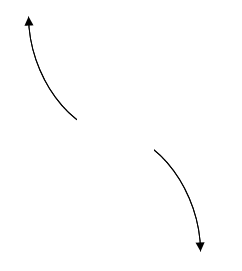
\includegraphics[width=0.3\textwidth]{../Figures/polyEndBehaviorAA.png}
    \end{center}\begin{enumerate}[label=\Alph*.]
\begin{multicols}{2}
\item 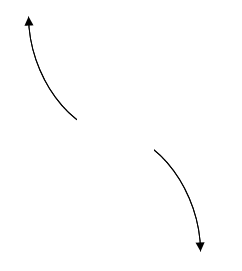
\includegraphics[width = 0.3\textwidth]{../Figures/polyEndBehaviorAA.png}
\item 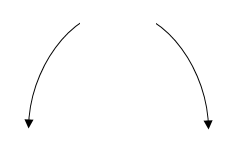
\includegraphics[width = 0.3\textwidth]{../Figures/polyEndBehaviorBA.png}
\item 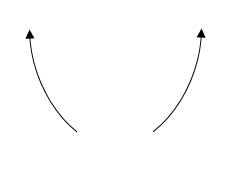
\includegraphics[width = 0.3\textwidth]{../Figures/polyEndBehaviorCA.png}
\item 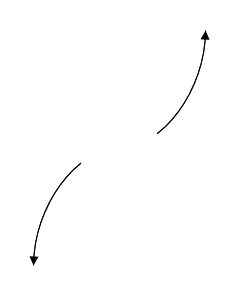
\includegraphics[width = 0.3\textwidth]{../Figures/polyEndBehaviorDA.png}
\end{multicols}\item None of the above.\end{enumerate}
\textbf{General Comment:} Remember that end behavior is determined by the leading coefficient AND whether the \textbf{sum} of the multiplicities is positive or negative.
}
\litem{
Construct the lowest-degree polynomial given the zeros below. Then, choose the intervals that contain the coefficients of the polynomial in the form $ax^3+bx^2+cx+d$.
\[ \frac{-6}{5}, \frac{3}{5}, \text{ and } \frac{7}{2} \]The solution is \( 50x^{3} -145 x^{2} -141 x + 126 \), which is option E.\begin{enumerate}[label=\Alph*.]
\item \( a \in [48, 54], b \in [-154, -139], c \in [-141, -135], \text{ and } d \in [-128, -118] \)

$50x^{3} -145 x^{2} -141 x -126$, which corresponds to multiplying everything correctly except the constant term.
\item \( a \in [48, 54], b \in [-206, -201], c \in [67, 73], \text{ and } d \in [125, 132] \)

$50x^{3} -205 x^{2} +69 x + 126$, which corresponds to multiplying out $(5x -6)(5x + 3)(2x -7)$.
\item \( a \in [48, 54], b \in [-267, -261], c \in [350, 357], \text{ and } d \in [-128, -118] \)

$50x^{3} -265 x^{2} +351 x -126$, which corresponds to multiplying out $(5x -6)(5x -3)(2x -7)$.
\item \( a \in [48, 54], b \in [142, 152], c \in [-141, -135], \text{ and } d \in [-128, -118] \)

$50x^{3} +145 x^{2} -141 x -126$, which corresponds to multiplying out $(5x -6)(5x + 3)(2x + 7)$.
\item \( a \in [48, 54], b \in [-154, -139], c \in [-141, -135], \text{ and } d \in [125, 132] \)

* $50x^{3} -145 x^{2} -141 x + 126$, which is the correct option.
\end{enumerate}

\textbf{General Comment:} To construct the lowest-degree polynomial, you want to multiply out $(5x + 6)(5x -3)(2x -7)$
}
\litem{
Describe the zero behavior of the zero $x = 5$ of the polynomial below.
\[ f(x) = -7(x - 3)^{6}(x + 3)^{3}(x - 5)^{10}(x + 5)^{7} \]The solution is the graph below, which is option B.
    \begin{center}
        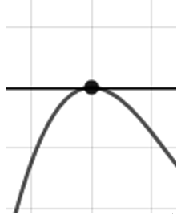
\includegraphics[width=0.3\textwidth]{../Figures/polyZeroBehaviorBA.png}
    \end{center}\begin{enumerate}[label=\Alph*.]
\begin{multicols}{2}
\item 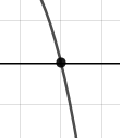
\includegraphics[width = 0.3\textwidth]{../Figures/polyZeroBehaviorAA.png}
\item 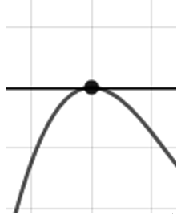
\includegraphics[width = 0.3\textwidth]{../Figures/polyZeroBehaviorBA.png}
\item 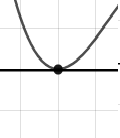
\includegraphics[width = 0.3\textwidth]{../Figures/polyZeroBehaviorCA.png}
\item 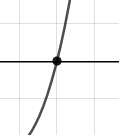
\includegraphics[width = 0.3\textwidth]{../Figures/polyZeroBehaviorDA.png}
\end{multicols}\item None of the above.\end{enumerate}
\textbf{General Comment:} You will need to sketch the entire graph, then zoom in on the zero the question asks about.
}
\litem{
Describe the end behavior of the polynomial below.
\[ f(x) = -8(x + 3)^{4}(x - 3)^{5}(x + 7)^{3}(x - 7)^{5} \]The solution is the graph below, which is option A.
    \begin{center}
        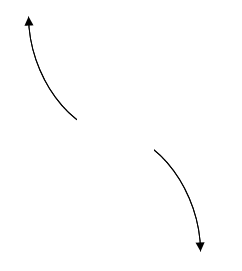
\includegraphics[width=0.3\textwidth]{../Figures/polyEndBehaviorCopyAA.png}
    \end{center}\begin{enumerate}[label=\Alph*.]
\begin{multicols}{2}
\item 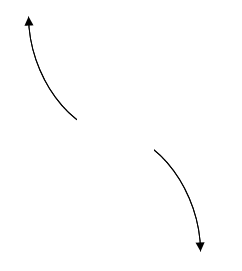
\includegraphics[width = 0.3\textwidth]{../Figures/polyEndBehaviorCopyAA.png}
\item 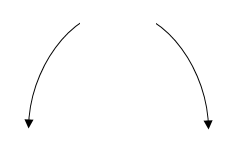
\includegraphics[width = 0.3\textwidth]{../Figures/polyEndBehaviorCopyBA.png}
\item 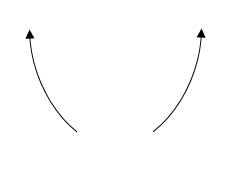
\includegraphics[width = 0.3\textwidth]{../Figures/polyEndBehaviorCopyCA.png}
\item 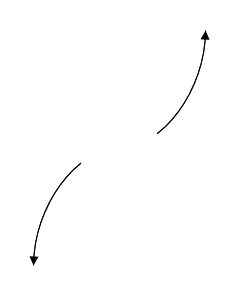
\includegraphics[width = 0.3\textwidth]{../Figures/polyEndBehaviorCopyDA.png}
\end{multicols}\item None of the above.\end{enumerate}
\textbf{General Comment:} Remember that end behavior is determined by the leading coefficient AND whether the \textbf{sum} of the multiplicities is positive or negative.
}
\litem{
Construct the lowest-degree polynomial given the zeros below. Then, choose the intervals that contain the coefficients of the polynomial in the form $x^3+bx^2+cx+d$.
\[ -5 + 5 i \text{ and } 3 \]The solution is \( x^{3} +7 x^{2} +20 x -150 \), which is option C.\begin{enumerate}[label=\Alph*.]
\item \( b \in [-11, -3], c \in [16, 22], \text{ and } d \in [145, 151] \)

$x^{3} -7 x^{2} +20 x + 150$, which corresponds to multiplying out $(x-(-5 + 5 i))(x-(-5 - 5 i))(x + 3)$.
\item \( b \in [1, 6], c \in [-1, 7], \text{ and } d \in [-18, -13] \)

$x^{3} + x^{2} +2 x -15$, which corresponds to multiplying out $(x + 5)(x -3)$.
\item \( b \in [2, 12], c \in [16, 22], \text{ and } d \in [-156, -141] \)

* $x^{3} +7 x^{2} +20 x -150$, which is the correct option.
\item \( b \in [1, 6], c \in [-9, 1], \text{ and } d \in [13, 20] \)

$x^{3} + x^{2} -8 x + 15$, which corresponds to multiplying out $(x -5)(x -3)$.
\item \( \text{None of the above.} \)

This corresponds to making an unanticipated error or not understanding how to use nonreal complex numbers to create the lowest-degree polynomial. If you chose this and are not sure what you did wrong, please contact the coordinator for help.
\end{enumerate}

\textbf{General Comment:} Remember that the conjugate of $a+bi$ is $a-bi$. Since these zeros always come in pairs, we need to multiply out $(x-(-5 + 5 i))(x-(-5 - 5 i))(x-(3))$.
}
\litem{
Which of the following equations \textit{could} be of the graph presented below?

\begin{center}
    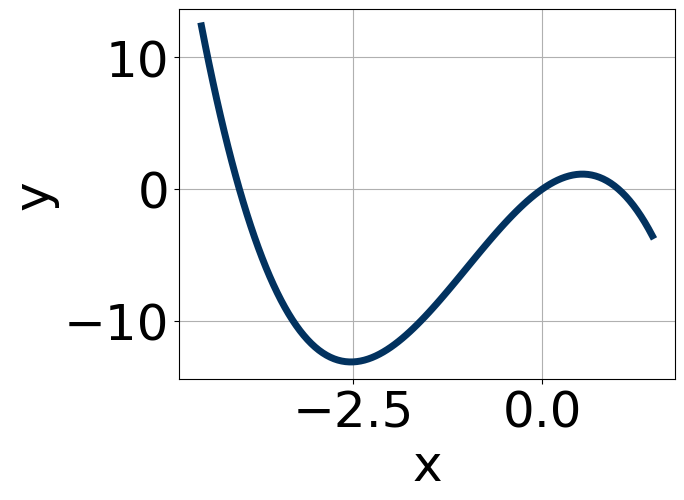
\includegraphics[width=0.5\textwidth]{../Figures/polyGraphToFunctionB.png}
\end{center}


The solution is \( -9x^{5} (x - 1)^{9} (x + 4)^{9} \), which is option A.\begin{enumerate}[label=\Alph*.]
\item \( -9x^{5} (x - 1)^{9} (x + 4)^{9} \)

* This is the correct option.
\item \( 17x^{11} (x - 1)^{9} (x + 4)^{9} \)

This corresponds to the leading coefficient being the opposite value than it should be.
\item \( 6x^{5} (x - 1)^{8} (x + 4)^{9} \)

The factor $(x - 1)$ should have an odd power and the leading coefficient should be the opposite sign.
\item \( -7x^{7} (x - 1)^{8} (x + 4)^{4} \)

The factors $1$ and $-4$ have have been odd power.
\item \( -17x^{7} (x - 1)^{10} (x + 4)^{9} \)

The factor $1$ should have been an odd power.
\end{enumerate}

\textbf{General Comment:} General Comments: Draw the x-axis to determine which zeros are touching (and so have even multiplicity) or cross (and have odd multiplicity).
}
\litem{
Which of the following equations \textit{could} be of the graph presented below?

\begin{center}
    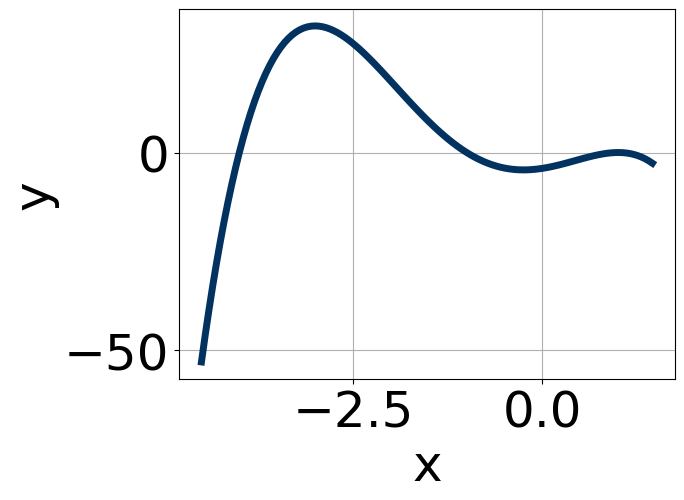
\includegraphics[width=0.5\textwidth]{../Figures/polyGraphToFunctionCopyB.png}
\end{center}


The solution is \( -4(x - 1)^{10} (x + 4)^{7} (x + 1)^{9} \), which is option E.\begin{enumerate}[label=\Alph*.]
\item \( -17(x - 1)^{4} (x + 4)^{8} (x + 1)^{9} \)

The factor $(x + 4)$ should have an odd power.
\item \( 20(x - 1)^{10} (x + 4)^{7} (x + 1)^{4} \)

The factor $(x + 1)$ should have an odd power and the leading coefficient should be the opposite sign.
\item \( 2(x - 1)^{10} (x + 4)^{9} (x + 1)^{9} \)

This corresponds to the leading coefficient being the opposite value than it should be.
\item \( -6(x - 1)^{7} (x + 4)^{8} (x + 1)^{11} \)

The factor $1$ should have an even power and the factor $-4$ should have an odd power.
\item \( -4(x - 1)^{10} (x + 4)^{7} (x + 1)^{9} \)

* This is the correct option.
\end{enumerate}

\textbf{General Comment:} General Comments: Draw the x-axis to determine which zeros are touching (and so have even multiplicity) or cross (and have odd multiplicity).
}
\litem{
Describe the zero behavior of the zero $x = -6$ of the polynomial below.
\[ f(x) = -4(x - 8)^{6}(x + 8)^{2}(x + 6)^{9}(x - 6)^{6} \]The solution is the graph below, which is option A.
    \begin{center}
        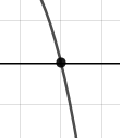
\includegraphics[width=0.3\textwidth]{../Figures/polyZeroBehaviorCopyAB.png}
    \end{center}\begin{enumerate}[label=\Alph*.]
\begin{multicols}{2}
\item 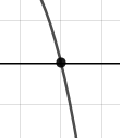
\includegraphics[width = 0.3\textwidth]{../Figures/polyZeroBehaviorCopyAB.png}
\item 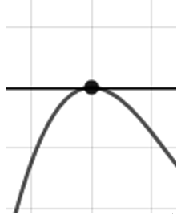
\includegraphics[width = 0.3\textwidth]{../Figures/polyZeroBehaviorCopyBB.png}
\item 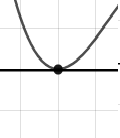
\includegraphics[width = 0.3\textwidth]{../Figures/polyZeroBehaviorCopyCB.png}
\item 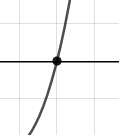
\includegraphics[width = 0.3\textwidth]{../Figures/polyZeroBehaviorCopyDB.png}
\end{multicols}\item None of the above.\end{enumerate}
\textbf{General Comment:} You will need to sketch the entire graph, then zoom in on the zero the question asks about.
}
\litem{
Construct the lowest-degree polynomial given the zeros below. Then, choose the intervals that contain the coefficients of the polynomial in the form $x^3+bx^2+cx+d$.
\[ -4 - 2 i \text{ and } -2 \]The solution is \( x^{3} +10 x^{2} +36 x + 40 \), which is option A.\begin{enumerate}[label=\Alph*.]
\item \( b \in [8, 13], c \in [34.2, 37], \text{ and } d \in [40, 42] \)

* $x^{3} +10 x^{2} +36 x + 40$, which is the correct option.
\item \( b \in [-4, 6], c \in [4.5, 8.2], \text{ and } d \in [6, 9] \)

$x^{3} + x^{2} +6 x + 8$, which corresponds to multiplying out $(x + 4)(x + 2)$.
\item \( b \in [-4, 6], c \in [3, 4.3], \text{ and } d \in [2, 5] \)

$x^{3} + x^{2} +4 x + 4$, which corresponds to multiplying out $(x + 2)(x + 2)$.
\item \( b \in [-14, -8], c \in [34.2, 37], \text{ and } d \in [-40, -32] \)

$x^{3} -10 x^{2} +36 x -40$, which corresponds to multiplying out $(x-(-4 - 2 i))(x-(-4 + 2 i))(x -2)$.
\item \( \text{None of the above.} \)

This corresponds to making an unanticipated error or not understanding how to use nonreal complex numbers to create the lowest-degree polynomial. If you chose this and are not sure what you did wrong, please contact the coordinator for help.
\end{enumerate}

\textbf{General Comment:} Remember that the conjugate of $a+bi$ is $a-bi$. Since these zeros always come in pairs, we need to multiply out $(x-(-4 - 2 i))(x-(-4 + 2 i))(x-(-2))$.
}
\litem{
Construct the lowest-degree polynomial given the zeros below. Then, choose the intervals that contain the coefficients of the polynomial in the form $ax^3+bx^2+cx+d$.
\[ \frac{-7}{5}, \frac{5}{2}, \text{ and } \frac{-1}{4} \]The solution is \( 40x^{3} -34 x^{2} -151 x -35 \), which is option D.\begin{enumerate}[label=\Alph*.]
\item \( a \in [35, 41], b \in [48, 58], c \in [-131, -125], \text{ and } d \in [-42, -32] \)

$40x^{3} +54 x^{2} -129 x -35$, which corresponds to multiplying out $(5x -7)(2x + 5)(4x + 1)$.
\item \( a \in [35, 41], b \in [-36, -27], c \in [-158, -150], \text{ and } d \in [33, 37] \)

$40x^{3} -34 x^{2} -151 x + 35$, which corresponds to multiplying everything correctly except the constant term.
\item \( a \in [35, 41], b \in [-148, -145], c \in [95, 106], \text{ and } d \in [33, 37] \)

$40x^{3} -146 x^{2} +101 x + 35$, which corresponds to multiplying out $(5x -7)(2x -5)(4x + 1)$.
\item \( a \in [35, 41], b \in [-36, -27], c \in [-158, -150], \text{ and } d \in [-42, -32] \)

* $40x^{3} -34 x^{2} -151 x -35$, which is the correct option.
\item \( a \in [35, 41], b \in [32, 40], c \in [-158, -150], \text{ and } d \in [33, 37] \)

$40x^{3} +34 x^{2} -151 x + 35$, which corresponds to multiplying out $(5x -7)(2x + 5)(4x -1)$.
\end{enumerate}

\textbf{General Comment:} To construct the lowest-degree polynomial, you want to multiply out $(5x + 7)(2x -5)(4x + 1)$
}
\litem{
Describe the end behavior of the polynomial below.
\[ f(x) = 8(x - 4)^{4}(x + 4)^{9}(x + 8)^{4}(x - 8)^{5} \]The solution is the graph below, which is option C.
    \begin{center}
        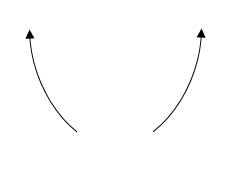
\includegraphics[width=0.3\textwidth]{../Figures/polyEndBehaviorCB.png}
    \end{center}\begin{enumerate}[label=\Alph*.]
\begin{multicols}{2}
\item 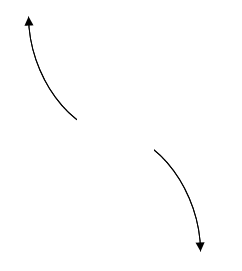
\includegraphics[width = 0.3\textwidth]{../Figures/polyEndBehaviorAB.png}
\item 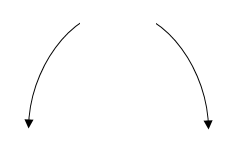
\includegraphics[width = 0.3\textwidth]{../Figures/polyEndBehaviorBB.png}
\item 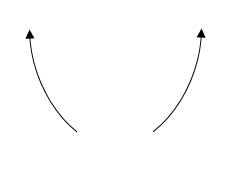
\includegraphics[width = 0.3\textwidth]{../Figures/polyEndBehaviorCB.png}
\item 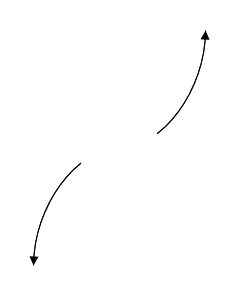
\includegraphics[width = 0.3\textwidth]{../Figures/polyEndBehaviorDB.png}
\end{multicols}\item None of the above.\end{enumerate}
\textbf{General Comment:} Remember that end behavior is determined by the leading coefficient AND whether the \textbf{sum} of the multiplicities is positive or negative.
}
\litem{
Construct the lowest-degree polynomial given the zeros below. Then, choose the intervals that contain the coefficients of the polynomial in the form $ax^3+bx^2+cx+d$.
\[ \frac{1}{2}, \frac{7}{4}, \text{ and } 4 \]The solution is \( 8x^{3} -50 x^{2} +79 x -28 \), which is option B.\begin{enumerate}[label=\Alph*.]
\item \( a \in [7, 12], b \in [-23, -12], c \in [-71, -59], \text{ and } d \in [-32, -21] \)

$8x^{3} -14 x^{2} -65 x -28$, which corresponds to multiplying out $(2x + 1)(4x + 7)(x -4)$.
\item \( a \in [7, 12], b \in [-51, -44], c \in [77, 82], \text{ and } d \in [-32, -21] \)

* $8x^{3} -50 x^{2} +79 x -28$, which is the correct option.
\item \( a \in [7, 12], b \in [49, 55], c \in [77, 82], \text{ and } d \in [28, 30] \)

$8x^{3} +50 x^{2} +79 x + 28$, which corresponds to multiplying out $(2x + 1)(4x + 7)(x + 4)$.
\item \( a \in [7, 12], b \in [-51, -44], c \in [77, 82], \text{ and } d \in [28, 30] \)

$8x^{3} -50 x^{2} +79 x + 28$, which corresponds to multiplying everything correctly except the constant term.
\item \( a \in [7, 12], b \in [-44, -34], c \in [31, 43], \text{ and } d \in [28, 30] \)

$8x^{3} -42 x^{2} +33 x + 28$, which corresponds to multiplying out $(2x + 1)(4x -7)(x -4)$.
\end{enumerate}

\textbf{General Comment:} To construct the lowest-degree polynomial, you want to multiply out $(2x -1)(4x -7)(x -4)$
}
\litem{
Describe the zero behavior of the zero $x = 2$ of the polynomial below.
\[ f(x) = -4(x - 2)^{5}(x + 2)^{10}(x - 3)^{6}(x + 3)^{10} \]The solution is the graph below, which is option A.
    \begin{center}
        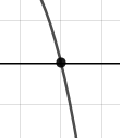
\includegraphics[width=0.3\textwidth]{../Figures/polyZeroBehaviorAB.png}
    \end{center}\begin{enumerate}[label=\Alph*.]
\begin{multicols}{2}
\item 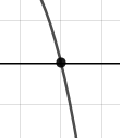
\includegraphics[width = 0.3\textwidth]{../Figures/polyZeroBehaviorAB.png}
\item 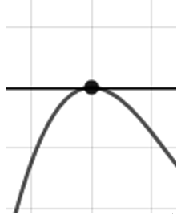
\includegraphics[width = 0.3\textwidth]{../Figures/polyZeroBehaviorBB.png}
\item 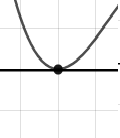
\includegraphics[width = 0.3\textwidth]{../Figures/polyZeroBehaviorCB.png}
\item 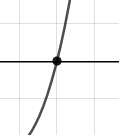
\includegraphics[width = 0.3\textwidth]{../Figures/polyZeroBehaviorDB.png}
\end{multicols}\item None of the above.\end{enumerate}
\textbf{General Comment:} You will need to sketch the entire graph, then zoom in on the zero the question asks about.
}
\litem{
Describe the end behavior of the polynomial below.
\[ f(x) = 2(x + 5)^{3}(x - 5)^{6}(x + 3)^{3}(x - 3)^{5} \]The solution is the graph below, which is option D.
    \begin{center}
        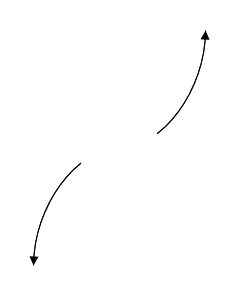
\includegraphics[width=0.3\textwidth]{../Figures/polyEndBehaviorCopyDB.png}
    \end{center}\begin{enumerate}[label=\Alph*.]
\begin{multicols}{2}
\item 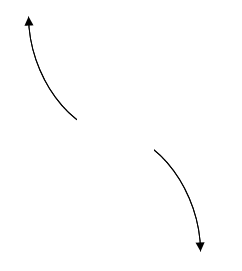
\includegraphics[width = 0.3\textwidth]{../Figures/polyEndBehaviorCopyAB.png}
\item 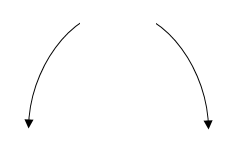
\includegraphics[width = 0.3\textwidth]{../Figures/polyEndBehaviorCopyBB.png}
\item 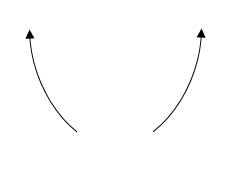
\includegraphics[width = 0.3\textwidth]{../Figures/polyEndBehaviorCopyCB.png}
\item 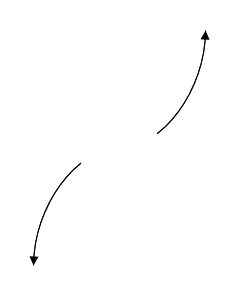
\includegraphics[width = 0.3\textwidth]{../Figures/polyEndBehaviorCopyDB.png}
\end{multicols}\item None of the above.\end{enumerate}
\textbf{General Comment:} Remember that end behavior is determined by the leading coefficient AND whether the \textbf{sum} of the multiplicities is positive or negative.
}
\litem{
Construct the lowest-degree polynomial given the zeros below. Then, choose the intervals that contain the coefficients of the polynomial in the form $x^3+bx^2+cx+d$.
\[ -2 - 5 i \text{ and } 3 \]The solution is \( x^{3} + x^{2} +17 x -87 \), which is option A.\begin{enumerate}[label=\Alph*.]
\item \( b \in [-0.9, 3.8], c \in [16, 20.1], \text{ and } d \in [-91, -82] \)

* $x^{3} + x^{2} +17 x -87$, which is the correct option.
\item \( b \in [-1.5, 0.8], c \in [16, 20.1], \text{ and } d \in [84, 91] \)

$x^{3} -1 x^{2} +17 x + 87$, which corresponds to multiplying out $(x-(-2 - 5 i))(x-(-2 + 5 i))(x + 3)$.
\item \( b \in [-0.9, 3.8], c \in [-3.2, -0.5], \text{ and } d \in [-6, -1] \)

$x^{3} + x^{2} -x -6$, which corresponds to multiplying out $(x + 2)(x -3)$.
\item \( b \in [-0.9, 3.8], c \in [0.2, 7.4], \text{ and } d \in [-15, -11] \)

$x^{3} + x^{2} +2 x -15$, which corresponds to multiplying out $(x + 5)(x -3)$.
\item \( \text{None of the above.} \)

This corresponds to making an unanticipated error or not understanding how to use nonreal complex numbers to create the lowest-degree polynomial. If you chose this and are not sure what you did wrong, please contact the coordinator for help.
\end{enumerate}

\textbf{General Comment:} Remember that the conjugate of $a+bi$ is $a-bi$. Since these zeros always come in pairs, we need to multiply out $(x-(-2 - 5 i))(x-(-2 + 5 i))(x-(3))$.
}
\litem{
Which of the following equations \textit{could} be of the graph presented below?

\begin{center}
    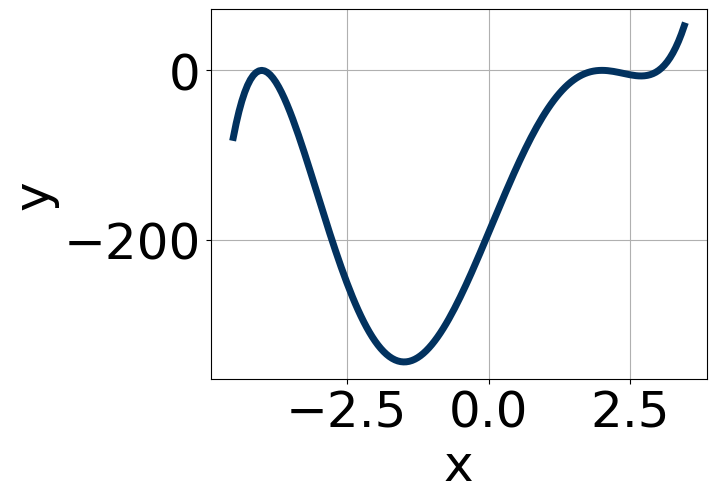
\includegraphics[width=0.5\textwidth]{../Figures/polyGraphToFunctionC.png}
\end{center}


The solution is \( 8(x + 4)^{6} (x - 2)^{8} (x - 3)^{9} \), which is option C.\begin{enumerate}[label=\Alph*.]
\item \( 13(x + 4)^{6} (x - 2)^{5} (x - 3)^{9} \)

The factor $(x - 2)$ should have an even power.
\item \( -18(x + 4)^{4} (x - 2)^{10} (x - 3)^{6} \)

The factor $(x - 3)$ should have an odd power and the leading coefficient should be the opposite sign.
\item \( 8(x + 4)^{6} (x - 2)^{8} (x - 3)^{9} \)

* This is the correct option.
\item \( 3(x + 4)^{8} (x - 2)^{9} (x - 3)^{4} \)

The factor $(x - 2)$ should have an even power and the factor $(x - 3)$ should have an odd power.
\item \( -8(x + 4)^{4} (x - 2)^{8} (x - 3)^{5} \)

This corresponds to the leading coefficient being the opposite value than it should be.
\end{enumerate}

\textbf{General Comment:} General Comments: Draw the x-axis to determine which zeros are touching (and so have even multiplicity) or cross (and have odd multiplicity).
}
\litem{
Which of the following equations \textit{could} be of the graph presented below?

\begin{center}
    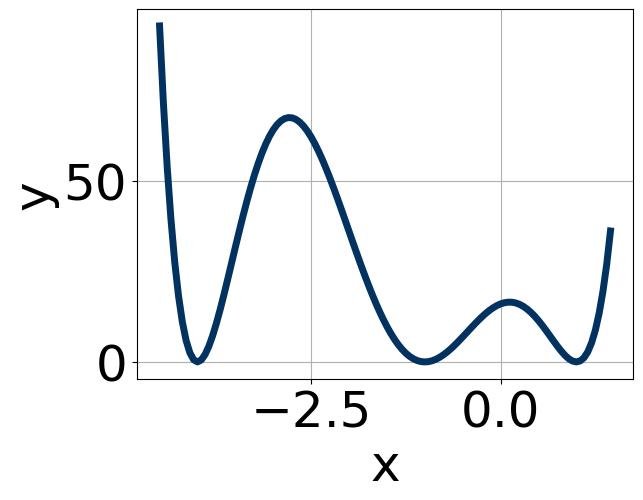
\includegraphics[width=0.5\textwidth]{../Figures/polyGraphToFunctionCopyC.png}
\end{center}


The solution is \( 18(x + 4)^{6} (x + 1)^{4} (x - 1)^{8} \), which is option C.\begin{enumerate}[label=\Alph*.]
\item \( -18(x + 4)^{10} (x + 1)^{4} (x - 1)^{8} \)

This corresponds to the leading coefficient being the opposite value than it should be.
\item \( 20(x + 4)^{8} (x + 1)^{5} (x - 1)^{7} \)

The factors $(x + 1)$ and $(x - 1)$ should both have even powers.
\item \( 18(x + 4)^{6} (x + 1)^{4} (x - 1)^{8} \)

* This is the correct option.
\item \( -4(x + 4)^{10} (x + 1)^{10} (x - 1)^{7} \)

The factor $(x - 1)$ should have an even power and the leading coefficient should be the opposite sign.
\item \( 6(x + 4)^{8} (x + 1)^{4} (x - 1)^{7} \)

The factor $(x - 1)$ should have an even power.
\end{enumerate}

\textbf{General Comment:} General Comments: Draw the x-axis to determine which zeros are touching (and so have even multiplicity) or cross (and have odd multiplicity).
}
\litem{
Describe the zero behavior of the zero $x = 6$ of the polynomial below.
\[ f(x) = -3(x + 4)^{8}(x - 4)^{5}(x + 6)^{6}(x - 6)^{5} \]The solution is the graph below, which is option A.
    \begin{center}
        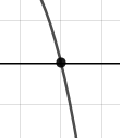
\includegraphics[width=0.3\textwidth]{../Figures/polyZeroBehaviorCopyAC.png}
    \end{center}\begin{enumerate}[label=\Alph*.]
\begin{multicols}{2}
\item 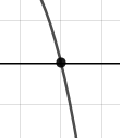
\includegraphics[width = 0.3\textwidth]{../Figures/polyZeroBehaviorCopyAC.png}
\item 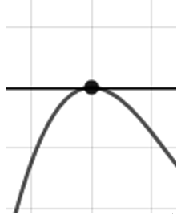
\includegraphics[width = 0.3\textwidth]{../Figures/polyZeroBehaviorCopyBC.png}
\item 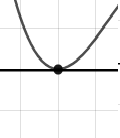
\includegraphics[width = 0.3\textwidth]{../Figures/polyZeroBehaviorCopyCC.png}
\item \includegraphics[width = 0.3\textwidth]{../Figures/polyZeroBehaviorCopyDC.png}
\end{multicols}\item None of the above.\end{enumerate}
\textbf{General Comment:} You will need to sketch the entire graph, then zoom in on the zero the question asks about.
}
\litem{
Construct the lowest-degree polynomial given the zeros below. Then, choose the intervals that contain the coefficients of the polynomial in the form $x^3+bx^2+cx+d$.
\[ -2 + 5 i \text{ and } 1 \]The solution is \( x^{3} +3 x^{2} +25 x -29 \), which is option A.\begin{enumerate}[label=\Alph*.]
\item \( b \in [2.3, 3.6], c \in [24, 32], \text{ and } d \in [-30, -20] \)

* $x^{3} +3 x^{2} +25 x -29$, which is the correct option.
\item \( b \in [-1.2, 1.7], c \in [-10, -3], \text{ and } d \in [0, 12] \)

$x^{3} + x^{2} -6 x + 5$, which corresponds to multiplying out $(x -5)(x -1)$.
\item \( b \in [-1.2, 1.7], c \in [-1, 13], \text{ and } d \in [-5, 0] \)

$x^{3} + x^{2} +x -2$, which corresponds to multiplying out $(x + 2)(x -1)$.
\item \( b \in [-5.5, -1.7], c \in [24, 32], \text{ and } d \in [23, 32] \)

$x^{3} -3 x^{2} +25 x + 29$, which corresponds to multiplying out $(x-(-2 + 5 i))(x-(-2 - 5 i))(x + 1)$.
\item \( \text{None of the above.} \)

This corresponds to making an unanticipated error or not understanding how to use nonreal complex numbers to create the lowest-degree polynomial. If you chose this and are not sure what you did wrong, please contact the coordinator for help.
\end{enumerate}

\textbf{General Comment:} Remember that the conjugate of $a+bi$ is $a-bi$. Since these zeros always come in pairs, we need to multiply out $(x-(-2 + 5 i))(x-(-2 - 5 i))(x-(1))$.
}
\litem{
Construct the lowest-degree polynomial given the zeros below. Then, choose the intervals that contain the coefficients of the polynomial in the form $ax^3+bx^2+cx+d$.
\[ 2, \frac{1}{5}, \text{ and } \frac{-1}{4} \]The solution is \( 20x^{3} -39 x^{2} -3 x + 2 \), which is option C.\begin{enumerate}[label=\Alph*.]
\item \( a \in [17, 29], b \in [-39.3, -36.6], c \in [-5.1, -0.4], \text{ and } d \in [-4, 0] \)

$20x^{3} -39 x^{2} -3 x -2$, which corresponds to multiplying everything correctly except the constant term.
\item \( a \in [17, 29], b \in [47.6, 51.5], c \in [18.7, 20.3], \text{ and } d \in [2, 8] \)

$20x^{3} +49 x^{2} +19 x + 2$, which corresponds to multiplying out $(x + 2)(5x + 1)(4x + 1)$.
\item \( a \in [17, 29], b \in [-39.3, -36.6], c \in [-5.1, -0.4], \text{ and } d \in [2, 8] \)

* $20x^{3} -39 x^{2} -3 x + 2$, which is the correct option.
\item \( a \in [17, 29], b \in [33.4, 40.5], c \in [-5.1, -0.4], \text{ and } d \in [-4, 0] \)

$20x^{3} +39 x^{2} -3 x -2$, which corresponds to multiplying out $(x + 2)(5x + 1)(4x -1)$.
\item \( a \in [17, 29], b \in [39.7, 41.9], c \in [-2, 2.2], \text{ and } d \in [-4, 0] \)

$20x^{3} +41 x^{2} +x -2$, which corresponds to multiplying out $(x + 2)(5x -1)(4x + 1)$.
\end{enumerate}

\textbf{General Comment:} To construct the lowest-degree polynomial, you want to multiply out $(x -2)(5x -1)(4x + 1)$
}
\litem{
Describe the end behavior of the polynomial below.
\[ f(x) = 5(x - 5)^{4}(x + 5)^{5}(x - 6)^{5}(x + 6)^{6} \]The solution is the graph below, which is option C.
    \begin{center}
        \includegraphics[width=0.3\textwidth]{../Figures/polyEndBehaviorCC.png}
    \end{center}\begin{enumerate}[label=\Alph*.]
\begin{multicols}{2}
\item \includegraphics[width = 0.3\textwidth]{../Figures/polyEndBehaviorAC.png}
\item \includegraphics[width = 0.3\textwidth]{../Figures/polyEndBehaviorBC.png}
\item \includegraphics[width = 0.3\textwidth]{../Figures/polyEndBehaviorCC.png}
\item \includegraphics[width = 0.3\textwidth]{../Figures/polyEndBehaviorDC.png}
\end{multicols}\item None of the above.\end{enumerate}
\textbf{General Comment:} Remember that end behavior is determined by the leading coefficient AND whether the \textbf{sum} of the multiplicities is positive or negative.
}
\litem{
Construct the lowest-degree polynomial given the zeros below. Then, choose the intervals that contain the coefficients of the polynomial in the form $ax^3+bx^2+cx+d$.
\[ -5, \frac{-2}{3}, \text{ and } \frac{-7}{5} \]The solution is \( 15x^{3} +106 x^{2} +169 x + 70 \), which is option E.\begin{enumerate}[label=\Alph*.]
\item \( a \in [12, 16], b \in [103, 110], c \in [161, 178], \text{ and } d \in [-74, -62] \)

$15x^{3} +106 x^{2} +169 x -70$, which corresponds to multiplying everything correctly except the constant term.
\item \( a \in [12, 16], b \in [-72, -57], c \in [-75, -65], \text{ and } d \in [68, 74] \)

$15x^{3} -64 x^{2} -69 x + 70$, which corresponds to multiplying out $(x -5)(3x -2)(5x + 7)$.
\item \( a \in [12, 16], b \in [-45, -43], c \in [-142, -136], \text{ and } d \in [-74, -62] \)

$15x^{3} -44 x^{2} -141 x -70$, which corresponds to multiplying out $(x -5)(3x + 2)(5x + 7)$.
\item \( a \in [12, 16], b \in [-113, -105], c \in [161, 178], \text{ and } d \in [-74, -62] \)

$15x^{3} -106 x^{2} +169 x -70$, which corresponds to multiplying out $(x -5)(3x -2)(5x -7)$.
\item \( a \in [12, 16], b \in [103, 110], c \in [161, 178], \text{ and } d \in [68, 74] \)

* $15x^{3} +106 x^{2} +169 x + 70$, which is the correct option.
\end{enumerate}

\textbf{General Comment:} To construct the lowest-degree polynomial, you want to multiply out $(x + 5)(3x + 2)(5x + 7)$
}
\litem{
Describe the zero behavior of the zero $x = -9$ of the polynomial below.
\[ f(x) = -9(x - 9)^{4}(x + 9)^{5}(x + 3)^{9}(x - 3)^{10} \]The solution is the graph below, which is option D.
    \begin{center}
        \includegraphics[width=0.3\textwidth]{../Figures/polyZeroBehaviorDC.png}
    \end{center}\begin{enumerate}[label=\Alph*.]
\begin{multicols}{2}
\item \includegraphics[width = 0.3\textwidth]{../Figures/polyZeroBehaviorAC.png}
\item \includegraphics[width = 0.3\textwidth]{../Figures/polyZeroBehaviorBC.png}
\item \includegraphics[width = 0.3\textwidth]{../Figures/polyZeroBehaviorCC.png}
\item \includegraphics[width = 0.3\textwidth]{../Figures/polyZeroBehaviorDC.png}
\end{multicols}\item None of the above.\end{enumerate}
\textbf{General Comment:} You will need to sketch the entire graph, then zoom in on the zero the question asks about.
}
\litem{
Describe the end behavior of the polynomial below.
\[ f(x) = 5(x - 5)^{5}(x + 5)^{10}(x - 8)^{5}(x + 8)^{7} \]The solution is the graph below, which is option D.
    \begin{center}
        \includegraphics[width=0.3\textwidth]{../Figures/polyEndBehaviorCopyDC.png}
    \end{center}\begin{enumerate}[label=\Alph*.]
\begin{multicols}{2}
\item \includegraphics[width = 0.3\textwidth]{../Figures/polyEndBehaviorCopyAC.png}
\item \includegraphics[width = 0.3\textwidth]{../Figures/polyEndBehaviorCopyBC.png}
\item \includegraphics[width = 0.3\textwidth]{../Figures/polyEndBehaviorCopyCC.png}
\item \includegraphics[width = 0.3\textwidth]{../Figures/polyEndBehaviorCopyDC.png}
\end{multicols}\item None of the above.\end{enumerate}
\textbf{General Comment:} Remember that end behavior is determined by the leading coefficient AND whether the \textbf{sum} of the multiplicities is positive or negative.
}
\end{enumerate}

\end{document}